%%%%%%%%%%%%%%%%%%%%%%%%%%%%%%%%%%%%%%%%%%%%%%%%%%%%%%%%%%%%%%%%%%%%%%%%%%%
%%%                                                                     %%%
%%%   LaTeX template voor het verslag van P&O: Computerwetenschappen.   %%%
%%%                                                                     %%%
%%%   Opties:                                                           %%%
%%%     tt      Tussentijdsverslag                                      %%%
%%%     eind    Eindverslag                                             %%%
%%%                                                                     %%%
%%%   3 oktober 2016                                   %%%
%%%   Versie 1.4                                                        %%%
%%%                                                                     %%%
%%%%%%%%%%%%%%%%%%%%%%%%%%%%%%%%%%%%%%%%%%%%%%%%%%%%%%%%%%%%%%%%%%%%%%%%%%%

\documentclass[tt]{penoverslag}
\usepackage{url}
\usepackage{amsmath}
\usepackage{caption}
\usepackage{subcaption}
\usepackage{amsmath,bm}


%%% PACKAGES %%%



\begin{document}

% == TITELPAGINA == %
\team{Zilver}
\year{2016-2017}
\members{Bram Vandendriessche (Co\"ordinator)\\
         Arne Vlietinck (Secretaris)\\
         Matthias Van der Heyden \\
         Jef Versyck\\
         Vincent Vliegen\\
         Laura Vranken}
\maketitlepage


% == SAMENVATTING == %
\begin{abstract}
\noindent {\em Auteurs: ; redactie: Arne Vlietinck}
\\


\end{abstract}


% == INHOUDSOPGAVE == %
\tableofcontents\newpage

%Dit zal dan verwijderd worden, wanneer het verslag volledig is.
%\em Enkele algemene richtlijnen : 
\begin{itemize}
\item Maak in het hele verslag gebruik van genummerde referenties, zoals hier ge\"\i llustreerd \cite{website:wikibooks-biblio}.  
\item Geef op het niveau van secties en/of subsecties aan wie de auteurs van dat deel zijn.  Een auteur is iemand die de tekst inhoudelijk en vormelijk mee bepaald heeft.    Als de secretaris of iemand anders de tekst vormelijk gewijzigd heeft, bv. om hem meer in lijn met de rest van het verslag te brengen, maar inhoudelijk niets toegevoegd heeft, is die persoon geen auteur maar een redacteur.  Je kan na de auteursnamen eventueel ``redactie: naam'' schrijven om aan te geven dat er substanti\"ele redactie gebeurd is (meer dan pakweg een paar tikfouten verbeteren).  Wanneer alle teamleden samen verantwoordelijk zijn voor een stuk (bv. samenvatting, conclusies) kan je de namen eventueel weglaten.
\item We verwachten dat alle groepsleden een substanti\"ele bijdrage leveren aan het  verslag, en dat dit ook zichtbaar is in de tekst!
\end{itemize}


\rm 

% == INLEIDING == %
\section*{Inleiding}
\label{sec:Inleiding}
\noindent {\em Auteurs: ; redactie: Arne Vlietinck}
\\


% == Beschrijving materiaal en bouw drone == %
\section{Ontwerp}
\label{sec:Ontwerp}

\subsection{Drone Autopilot}
\label{subsec:OntwerpAutopilot}
\noindent
Ten eerste moeten de beelden die de Autopilot van de Virtual Testbed binnenkrijgt, geanalyseerd worden. Dit gebeurt door iteratief de kleurwaarden van elke pixel te vergelijken met de waarde van de opgegeven kleur. Deze methode wordt logischerwijs enkel gebruikt indien er al een doelkleur beslist is. Anders zullen de pixels gegroepeerd worden per kleur die voorkomt in een \textit{HashMap}. De gekleurde pixels worden bijgehouden door hun positie ten opzichte van het beeld, uitgedrukt in rij en kolom. De berekeningen worden gebaseerd op het midden van de bol. Dit kan benaderd worden op twee manieren: via het zwaartepunt of de kleinste-kwadratenmethode op de randpunten van de cirkel. Het zwaartepunt van een bepaalde kleur pixels is te berekenen via het gemiddelde van de opgeslagen co\"ordinaten. De kleinste-kwadratenmethode zoekt daarentegen eerst de randpunten uit van de cirkel. Deze worden vervolgens gebruikt in het zoekalgoritme (zie sectie \ref{subsec: Kleinste kwadraten circle fit}) dat de cirkel bepaalt die het beste past in de gegeven randpunten. Hieruit kan dan de positie van het centrum van de bol bepaald worden. De Autopilot zal eerst gebruik maken van de kleinste-kwadratenmethode en overschakelen op de zwaartepuntberekening wanneer er onvoldoende randpunten zijn, aangezien deze minder nauwkeurig is wanneer het middelpunt buiten beeld ligt.
\\
Indien de Autopilot geen gekleurde pixels detecteert, zal de drone systematisch de wereld scannen. Hierover meer info in sectie \ref{subsec: Scannen wereld}.
%TODO: Vectoren -> @Vincent
%TODO: afremmen -> @Matthias
%TODO: polyhedra calculation -> @Laura
%TODO: scannen 1) tekenen; 2) idee -> @Bram & @Laura

\subsection{Virtual Testbed}
%TODO: Tekenen polyhedron -> @Bram
\subsection{Polyhedra en het bestaande ontwerp}
\noindent {\em Auteur: Bram Vandendriessche}
\\\\
Het ontwerp van de simulator zorgt ervoor dat de uitbreiding ervan met polyhedra vrij eenvoudig in te voeren is. Door het nieuwe type Polyhedron dat erft van de \textit{WorldObjects}, moesten in \textit{World} zelf slechts enkele extra methodes worden ge\"implementeerd m.b.t. het toevoegen en verwijderen van een Polyhedron aan de bestaande wereld.\\
\noindent
Het ontwerp van het Testbed heeft de grote zwakte dat het erg moeilijk is om individuele elementen en methodes te testen. Dit komt doordat de objecten vaak erg afhankelijk zijn van de wereld waarin ze bestaan. Die wereld is bovendien altijd afhankelijk van de \textit{gl}-component van OpenGL, waardoor het noodzakelijk is een volledige wereld op te zetten voor de test kan worden uitgevoerd. Een oplossing hiervoor zou zijn om de objecten en wereld zo op te splitsen dat presentatie en representatie gesplitst worden, zodat het representatie-gedeelte onafhankelijk kan gebruikt worden. Daarnaast zou dan enkel de wereld weet moeten hebben van haar objecten en niet andersom, zodat objecten onafhankelijk van de wereld kunnen worden getest.\\
\\
\noindent 
De Polyhedron zelf is zo ontworpen dat die bestaat uit verschillende Triangles. De tekenfunctie van de Polyhedron draagt elke Triangle die tot de Polyhedron behoort, op om zichzelf te tekenen. Een Triangle bestaat uit co\"ordinaten voor zijn drie hoekpunten en een kleur voor het buitenste gedeelte van de driehoek. Op basis daarvan worden de binnenste hoekpunten berekend en er wordt een kleur afgeleid uit de gegeven kleur zodat de driehoek voldoet aan de gegeven beperkingen m.b.t. de kleur, zie Tabel \ref{table: HSVwaarden}, en de oppervlakte.\\
\\
\noindent
Voor het testen van de Autopilot zijn verschillende figuren ontworpen. Zij vallen onder de \textit{PredefinedPolyhedron}, een subklasse van Polyhedron die ook een positie mee kan krijgen bij creatie. Hierdoor kan de figuur op een gewenste positie worden geplaatst. De standaard Polyhedra krijgen geen positie mee. Hun positie wordt gezet op het massapunt van de polyhedron (de gemiddelde 3D-co\"ordinaat van alle hoekpunten). Op die manier wordt gezorgd dat de positie logisch is t.o.v. de hoekpunten en het niet mogelijk is dat een figuur bijvoorbeeld rond (20,0,0) wordt gedefinieerd, maar wel een positie van (0,0,-40) krijgt toegewezen. De figuren vari\"eren van een eenvoudige met vier hoekpunten tot meer complexe zoals een kubus met een opening in, waarbij de Autopilot zal moeten weten dat het voor de drone niet mogelijk is hierdoor te vliegen, zie Figuur \ref{fig: polyhedra}.

\begin{figure}[h]
	\centering
	\begin{subfigure}{.5\textwidth}
		\centering
		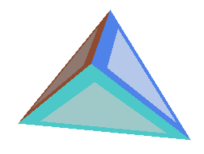
\includegraphics[width=.4\linewidth]{4point.png}
		\caption{Eenvoudige figuur}
	\end{subfigure}%
	\begin{subfigure}{.5\textwidth}
		\centering
		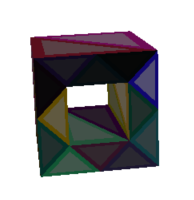
\includegraphics[width=.4\linewidth]{hollowcube.png}
		\caption{Complexere figuur}
	\end{subfigure}
	\caption{Voorgedefinieerde polyhedra.}
	\label{fig: polyhedra}
\end{figure}

%TODO: Generator/parser -> @Jef


% == ALGORITMES == %
\section{Algoritmes}
\label{sec:Algoritmes}

\subsection{Drone Autopilot}
\label{sec:AlgoritmesAutopilot}
%RotatieMatrixen
\subsubsection{Rotatiematrix}
\noindent {\em Auteur: Laura Vranken; redactie: Arne Vlietinck}
\\\\
Na een uitgebreide wijziging van de opgave werden de rotatiematrixen opnieuw opgesteld. De conventies in de nieuwe opgave komen niet overeen met de algemene conventies in de literatuur. Hierdoor werden de rotatiematrixen met extra zorg opgesteld. Het is een cruciaal element voor de ori\"entatie en bewegingen van de drone.

\begin{figure}[h!]
	\centering
		\(
		\begin{bmatrix} 
			cos(y) & 0 & -sin(y) \\ 
			0 & 1 & 0 \\
			sin(y) & 0 & cos(y)
		\end{bmatrix}
		\begin{bmatrix} 
			1 & 0 & 0 \\ 
			0 & cos(p) & sin(p) \\
			0 & -sin(p) & cos(p)
		\end{bmatrix}
		\begin{bmatrix} 
			cos(r) & sin(r) & 0 \\ 
			-sin(r) & cos(r) & 0 \\
			0 & 0 & 1
		\end{bmatrix}
		\)
	\caption{Bovenstaande matrixen geven respectievelijk de yaw-, pitch- en rollmatrix weer.}
\end{figure}
\noindent
Bovenstaande matrixen worden vermenigvuldigd in omgekeerde volgorde dit door de conventies van de rotatiematrixen. Met deze rotatiematrix kan ook de inverse berekend worden.
%TODO: Vectorberekeningen -> @Vincent

\subsection{Virtual Testbed}


% == SOFTWARE == %
\section{Software}
\label{sec:Software}

\subsection{Drone Autopilot}

\subsection{Virtual Testbed}


% == Testen == %
\section{Testen}
\label{sec:Testen}

% == BESLUIT == %
\section*{Besluit}
\label{sec:Besluit}
\noindent {\em Auteurs: ; redactie: Arne Vlietinck}
\\

% == REFERENTIES == %
\bibliographystyle{siam}
\bibliography{references.bib}


% == APPENDICES == %
%\newpage\makeappendix


%\section{MOET NOG WEG}
%De volgende informatie wordt na de finale demonstratie apart ingediend.

\section{Beschrijving van het proces}
\begin{itemize}
\item Welke moeilijkheden heb je ondervonden tijdens de uitwerking?
\item Welke lessen heb je getrokken uit de manier waarop je het project hebt aangepakt?
\item Hoe verliep het werken in team? Op welke manier werd de teamco\"ordinatie en planning aangepakt?
\end{itemize}


\section{Beschrijving van de werkverdeling}
\begin{itemize}
\item Geef voor elk van de groepsleden aan aan welke delen ze hebben meegewerkt en welke andere taken ze op zich hebben genomen.
\item Rapporteer in tabelvorm hoeveel uur elk groepslid elke week aan het project gewerkt heeft, zowel tijdens als buiten de begeleide sessies. Geef ook totalen per groepslid voor het volledige semester.
\end{itemize}


\section{Kritische analyse}
\begin{itemize}
\item Maak een analyse van de sterke en zwakke punten van het project. Welke punten zijn vatbaar voor verbetering. Wat zou je, met je huidige kennis, anders aangepakt hebben?
\end{itemize}



\end{document}
